\documentclass{article}
\usepackage[utf8]{inputenc}
\usepackage{indentfirst}
\usepackage{graphicx}
%\usepackage{biblatex}
%\addbibresource{allreferences.bib}

\title{\Large{EP2} \\ \Large{Numerical Integration using Monte Carlos Methods} \\ \small{Comparing quasi-random and pseudo-random numbers efficiency}}
\author{André Vinícius Rocha Pires \\ 10737290}
\date{April 2019}

\begin{document}

\maketitle

\section{Introduction}
This report is the third of a series on the experience of applying Monte Carlos Methods in numerical integration. The previous challenge were to calculate the integral with a good precision, defining the stopping criteria which satisfies it, i.e. the minimum number of samples necessary to get the value of the integral with a given precision. Now, all the processes were repeated using quasi-random number generation instead of pseudo-random. Again, the applied methods were:

\begin{itemize}
    \item Crude
    \item Hit-and-miss
    \item Importance Sampling
    \item Control Variate
\end{itemize}

A complete explanation about the tests implementation and math functions applied will be given. Then, we will produce data for a table with means and dispersion of the $'n'$ for each method and random generator. As a conclusion, comparisons between quasi and pseudo-random about the necessary number of samples will show its differences.

\section{The Math and the Code}

Initially, a R function for each of the methods was defined. As some of these methods have an auxiliary math function, here we will document the math and the code together. 

\subsection{Crude Monte Carlos}

\begin{itemize}
    \item \textbf{Description}\newline
    Are inserted $n$ random values as $x \sim U(0, 1)$ in a function $f(x)$ defined in $[0,1]$. The mean of $f(x)$ is our integral.
    
    \item \textbf{Math}\newline
    The Mean Value Theorem is the basis for this method.
    
    \item \textbf{Usage}\newline
    mc\_crude(intfunc, n, seed, usequasi = TRUE)
    
    \item \textbf{Arguments}
    
    \begin{itemize}
        \item intfunc:   the function to integrate
        \item n:         the number of samples to use
        \item seed:      optional. For the random number generator
        \item usequasi:  logic. Use quasi-random numbers or not. Default TRUE.
    \end{itemize}

\end{itemize}

\subsection{Hit-or-Miss Monte Carlos}

\begin{itemize}
    \item \textbf{Description}\newline
    Are inserted $n$ random values as $x \sim U(0, 1)$ in a function $f(x)$ defined in $[0,1]$. These values are compared with other $n$ random values as $y \sim U(0, 1)$. If $y \leq f(x)$, we count an hit. The integral is the ratio between the hits and the $n$ tries.
    
    \item \textbf{Math}\newline
    The basis for this method is Geometric Probability. The ratio we are really comparing is the area under the curve versus the interval of our 1x1 square(the sample space).
    
    \item \textbf{Usage}\newline
    mc\_hitandmiss(intfunc, n, seed, usequasi = "yzes")
    
    \item \textbf{Arguments}
    \begin{itemize}
        \item intfunc:   the function to integrate
        \item n:         the number of samples to use
        \item seed:      optional. For the random number generator
        \item usequasi:  this is the only method where this argument is not logic. Here we can choose how we will use the quasi-random numbers: on $x$("xzes"), $y$("yzes"), "both" $x$ and $y$, or "none". Default "yzes".
    \end{itemize}
    \item \textbf{Details}\newline
    This method is the one which shows the most curious behaviours. For example, setting a seed for pseudo-random numbers will produce the same sequence. The choice of "yzes" as default was for efficiency purposes and its results will be shown at the end of this report.
\end{itemize}

\subsection{Importance Sampling Monte Carlos}

\begin{itemize}
    \item \textbf{Description}\newline
    Are inserted $n$ random values as $x \sim G$ in a function $f(x)$ defined in $[0,1]$. The mean of $f(x)/G(x)$ is our integral.
    
    \item \textbf{Math}\newline
    The method efficiency comes from using a density function $G$ that imitates the curves of the function $f$. This way, the samples got from $f(x)$ are proportionally frequent to your amplitude.
    
    \item \textbf{Usage}\newline
    mc\_importancesampling(intfunc, n, seed, usequasi = TRUE)
    
    \item \textbf{Arguments}
    
    \begin{itemize}
        \item intfunc:   the function to integrate
        \item n:         the number of samples to use
        \item seed:      optional. For the random number generator
        \item usequasi:  logic. Use quasi-random numbers or not. Default TRUE.
    \end{itemize}
    \item \textbf{Details}\newline
    For this method to fit with my $f$ function, I had to make some calculations to define a good $G$ function. As the $f$ function I got was almost an line in our interval, I got its ends and traced one linear function $g$, with:
    \begin{itemize}
        \item $g(0) = f(0) = 1$
        \item $g(1) = f(1) = 0.730945$
        \item $g(x) = f(0) - (1 - f(1))x = 1 - 0.269055x$
    \end{itemize}
    Integrating this function I got $G^*(x)$. Then I could know how much I had to sum to get an density function:
    \begin{itemize}
        \item $g(x) = 1 - 0.269055x$
        \item $G^*(x) = \int g(x)dx$
        \item $\int_0^1G^*(x)dx = 0.8654725$
        \item $1 - \int_0^1G^*(x)dx = 0.1345275$
        \item $g^*(x) = 1.1345275 - 0.269055x$
        \item $\int_0^1g^*(x)dx = 1$
        \item $\int g^*(x)dx = G(x) = 1.1345275x - 0.269055x^2/2$
    \end{itemize}
    At last, I got its inverse with Bhaskara from the formula:
    \begin{equation}
    x = \frac{-b \pm \sqrt{b^2 - 4ac}}{2a} \Rightarrow
    x_1 = G^{-1}(y) = \frac{-b - \sqrt{b^2 - 4a(c-y)}}{2a}
    \end{equation}
    \end{itemize}

\subsection{Control Variate Monte Carlos}

\begin{itemize}
    \item \textbf{Description}\newline
    Are inserted $n$ random values as $x \sim U(0, 1)$ in a function $f(x)$ defined in $[0,1]$. The mean of $f(x)$ is our integral.
    
    \item \textbf{Math}\newline
    In this method, the efficiency is got from using the most similar function to $f$ which we can integrate. Next, we apply Crude Monte Carlos on both. Then, we use the difference between the Monte Carlos integration and the real integration of our auxiliary function to correct our $f$
    
    \item \textbf{Usage}\newline
    mc\_controlvariate(intfunc, n, seed, usequasi = TRUE)
    
    \item \textbf{Arguments}
    
    \begin{itemize}
        \item intfunc:   the function to integrate
        \item n:         the number of samples to use
        \item seed:      optional. For the random number generator
        \item usequasi:  logic. Use quasi-random numbers or not. Default TRUE.
    \end{itemize}
    
    \item Details
    For this method I used the same $g$ function presented in Importance Sampling Monte Carlos.
    
\end{itemize}

\subsection{Defining the Stopping Criteria}
The problem of defining the stopping criteria was solved with a R function that recursively executes the methods functions, until it reaches a mathematical stopping criteria.

\begin{itemize}
\item \textbf{Description}\newline
    This R function calculates the integral of a math function $f(x)$ based on precision criteria given by the arguments. To do this, is implemented a loop with a stopping criteria that depends on an error tax. This error tax is calculated empirically, with the data produced by the function itself. The returned data, besides the resulting integral, shows the efficiency of the applied method through the number of iterations, the variance reduction and the estimated error tax:
    \begin{itemize}
        \item n              : the minimum necessary number of iterations for a given error tolerance
        \item variance       : the variance achieved
        \item expected\_value: the integral desired      
        \item error          : the estimated error tax
    \end{itemize}
    
    \item \textbf{Usage}\newline
monte\_carlos(intfunc, method, CI = 0.95, errtolerance = 0.01, ...)    
    \item \textbf{Arguments}
    
    \begin{itemize}
        \item intfunc: the function to integrate
        \item method: the Monte Carlos method applied
        \item CI: the confidence interval used to define the error
        \item errtolerance: the wanted precision
        \item (...)seed: optional. For the random number generator
        \item (...)usequasi: optional. See Monte Carlos methods documentation
    \end{itemize}
    
    \item \textbf{Math}\newline
Let be $f(x), x \in [0,1]$ our function, and $\gamma = \int_{0}^{1}f(x)dx$ the value of its integral. If $\hat{\gamma}$ is the estimated value, the wanted precision level is:

\begin{equation}
    \frac{\mid\hat{\gamma}-\gamma\mid}{\gamma} < 1\%
\label{eq:precisionlevel}
\end{equation}

Here, we have the problem of not knowing the real value of $\gamma$. Being that $\hat{\gamma}$ is an unbiased estimator for $\gamma$ in all the given methods, we will use as our best information:

\begin{equation}
    E[\hat{\gamma}] = \gamma
\label{eq:bestgamma}
\end{equation}

For the difference between the estimator and the real value of our integral, we applied an confidence interval. Here we can securely define to be the worst scenario when the difference is, for a given $n$:

\begin{equation}
    (E_n[\hat{\gamma}] + \epsilon_n) - 
    (E_n[\hat{\gamma}] - \epsilon_n) =
    2 \epsilon_n
\label{eq:worsterror}
\end{equation}

\begin{center}
    with $\epsilon_n = Z \times S_n(\hat{\gamma})/\sqrt{n}$
\end{center}

\begin{equation}
    \epsilon_n = Z \times S_n(\hat{\gamma})/\sqrt{n}
\end{equation}


Finally, applying \ref{eq:worsterror} and \ref{eq:bestgamma} to \ref{eq:precisionlevel}, our stopping criteria is to get the least $n$ that satisfies:

\begin{equation}
    \frac{2 \epsilon_n}{E_n[\hat{\gamma}]} < 0.01
\label{eq:stoppingcriteria}
\end{equation}



\end{itemize}


\section{Conclusion - Comparing results}
At last, for comparing results, a loop was implemented to produce data for our brief descriptive analysis. The table is sorted by mean.

\begin{center}
\begin{tabular}{ c c c c c c c}
METHOD & MIN  &  Q1 & MEDIAN & MEAN & Q3 & MAX \\
pseudo control & 2.00 & 2.00 & 2.00 & 2.26 & 2.00 & 4.00 \\
quasi control & 2.0 & 2.0 & 2.0 & 2.3 & 3.0 & 4.0 \\
quasi importance & 10.00 & 12.50 & 19.00 & 19.06 & 24.00 & 31.00 \\
pseudo importance & 2.00 & 24.00 & 28.00 & 26.27 & 33.00 & 43.00 \\
quasi crude & 21.00 & 40.75 & 46.00 & 45.49 & 51.00 & 71.00 \\
pseudo crude & 2.00 & 68.75 & 78.50 & 74.98 & 86.00 & 104.00 \\
Y hit-miss &  205.0 & 244.0 & 261.0 & 277.4 & 285.5 & 493.0 \\
X hit-miss & 299.0 & 336.0 & 361.0 & 389.8 & 406.8 & 597.0 \\
NONE hit-miss & 298.0 & 347.0 & 377.0 & 403.5 & 415.5 & 635.0 \\
XY hit-miss & 445.0 & 476.0 & 492.5 & 509.4 & 519.2 & 683.0
 \end{tabular}
\end{center}

\begin{figure}[htbp]
\begin{center}
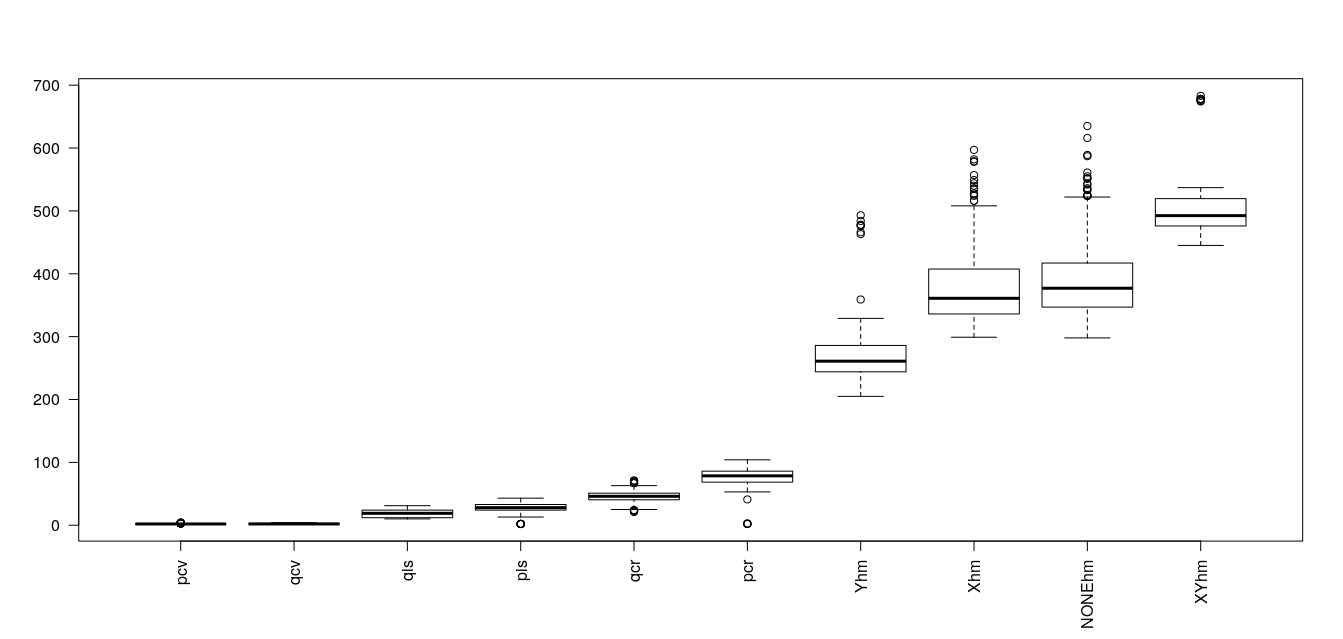
\includegraphics[width=0.8\paperwidth]{Rplot01.png}
\end{center}
\label{fig:boxplots}
\end{figure}
%\printbibliography

\end{document}